\documentclass[11pt]{article}

\usepackage{amsmath}
\usepackage{amssymb}
\usepackage{fancyhdr}
\usepackage{comment}
\usepackage{color}
\usepackage{graphicx}
\usepackage[colorlinks=true,linkcolor=blue,urlcolor=blue]{hyperref}

\newcounter{marks}
\def\maxmarks#1{\extramark{#1}\addtocounter{marks}{#1}}
\def\extramark#1{
  \begin{flushright}
  [\emph{#1 points}]
  \end{flushright}
%  \quad\mbox{\LARGE\begin{tabular}{|c|c|}
%  \hline\rule{1cm}{0cm} & #1 \\ \hline \end{tabular}}
}
\def\dumptotal{%
\begin{flushright}
\begin{tabular}{|l|} \hline
\LARGE{\textbf{\rule{0pt}{16pt}Total:~\themarks}} \\ \hline
\end{tabular}
\end{flushright}}
\def\skiplines#1{\newline \forloop{#1}{{\rule{0pt}{20pt}} \\}}

\specialcomment{answer}{\color{blue}}{\color{black}}
\def\withanswers{\def\skiplines##1{\relax}\def\skippage{\relax}}
\def\withoutanswers{\excludecomment{answer}\def\skippage{\clearpage}}

\newif\ifprint
\printtrue

\oddsidemargin0cm
\topmargin-2cm     %I recommend adding these three lines to increase the 
\textwidth16.5cm   %amount of usable space on the page (and save trees)
\textheight23.5cm  

\newcommand{\mycoursenum}{10-601}
\newcommand{\myhwnum}{2}
\newcommand{\myname}{Your Name Here}
\newcommand{\myandrew}{your-andrew-id-here@andrew.cmu.edu}
\newcommand{\myfirstta}{Siddhartha Jain}
\newcommand{\mysecondta}{Ying Yang}

\newcommand{\question}[2] {\vspace{.25in} \hrule\vspace{0.5em} \noindent{\bf #1: #2} \vspace{0.5em} \hrule \vspace{.10in}}
\renewcommand{\part}[1] {\vspace{.10in} {\bf (#1)}}

\setlength{\parindent}{0pt}
\setlength{\parskip}{5pt plus 1pt}
 
\pagestyle{fancyplain}
\lhead{\fancyplain{}{\textbf{HW\myhwnum}}}
\ifprint
\rhead{\fancyplain{}{Andrew ID: \rule{0.2\textwidth}{.4pt}}}
\else
\rhead{\fancyplain{}{\myname\\ \myandrew}}
\fi
\chead{\fancyplain{}{\mycoursenum}}

\withoutanswers

\begin{document}

\medskip

\thispagestyle{plain}
\begin{center}
{\Large \mycoursenum: Homework \myhwnum} \\
Due: 25 September 2014 11:59pm (Autolab) \\
TAs: \myfirstta, \mysecondta \\
\medskip
\ifprint
Name: \rule{0.5\textwidth}{.4pt} \\
Andrew ID: \rule{0.45\textwidth}{.4pt} \\
\else
Name: \myname \\
Andrew ID: \myandrew \\
\fi
\end{center}

Please answer to the point, and do not spend time/space giving irrelevant details. 
%You should not require more space than is provided for each question. If you do, please think whether you can make your argument more pithy, an exercise that can often lead to more insight into the problem. 
Please state any additional assumptions you make while answering the questions. 
For Questions 1 to 5, 6(b) and 6(c), you need to submit your answers in a single PDF file on autolab, either a scanned handwritten version or a \LaTeX pdf file. 
Please make sure you write legibly for grading.
For Question 6(a), submit your m-files on autolab. 

You can work in groups. However, no written notes can be shared, or taken during group discussions. You may ask clarifying questions on Piazza. However, under no circumstances should you reveal any part of the answer publicly on Piazza or any other public website. The intention of this policy is to facilitate learning, not circumvent it. Any incidents of plagiarism will be handled in accordance with \href{http://www.cmu.edu/policies/documents/Academic%20Integrity.htm}{CMU's Policy on Academic Integrity}.


%%%%%%%%%%%%%%%%%%%%%%%%%%%%%%%%%%%%%%%%%%%
\question{$\star$}{Code of Conduct Declaration}

\begin{itemize}
	\item Did you receive any help whatsoever from anyone in solving this assignment? Yes / No.
	\item If you answered \emph{yes}, give full details: \rule{0.4\textwidth}{.4pt} (e.g. \emph{Jane explained to me what is asked in Question 3.4})
	\item Did you give any help whatsoever to anyone in solving this assignment? Yes / No.
	\item If you answered \emph{yes}, give full details: \rule{0.4\textwidth}{.4pt} (e.g. \emph{I pointed Joe to section 2.3 to help him with Question 2}).
\end{itemize}


\clearpage
%%%%%%%%%%%%%%%%%%%%%%%%%%%%%%%%%%%%%%%%%%%
\question{1}{A probabilistic view of linear regression. (TA:- \mysecondta)}
Let $X$ and $Y$  be two random variables,  $\beta$ be a constant, and $\epsilon \sim \mathcal{N}(0, \sigma^2)$ be a Gaussian random variable with zero mean and variance $\sigma^2$. 
We assume $Y = \beta X + \epsilon$, and that $\epsilon$ is independent of $X$.  \\

\part{a} Show that given $X = x$, the distribution of $Y$ is $\mathcal{N}(\beta x, \sigma^2)$
\maxmarks{3} \vspace*{1.35 cm}

\part{b} Let $\{(X_i, Y_i),i = 1, \cdots, n\}$ be $n$ independent samples from the model above. 
     Show that the maximum likelihood estimation of $\beta$, where the likelihood is with regard to the conditional distribution $Y|X$, is the least square solution
    \begin{align*}
    \hat\beta = \arg\min_{\beta}  \sum_{i=1}^{n} (Y_i - \beta X_i)^2
    \end{align*}
\maxmarks{3} \vspace*{3 cm}


\clearpage

%%%%%%%%%%%%%%%%%%%%%%%%%%%%%%%%%%%%%%%%%%%
\question{2}{One-dimensional ridge regression(TA:- \mysecondta)}

Let $Y$ and $X$ be two random variables, and $Y = \beta X + \epsilon$ given $X$, where $\beta$ is a constant, and $\epsilon \sim \mathcal{N}(0,\sigma^2)$, independent of $X$. 
Given $n$ independent sample pairs, $(x_1, y_1), (x_2, y_2), \cdots, (x_n, y_n)$,
instead of ordinary least square, here we estimate $\beta$ with ``ridge regression'', by solving the following problem. 
\begin{align*}
\hat{\beta} = \arg \min_{\beta}\frac{1}{2}\left(\sum_{i=1}^n(y_i- \beta x_i)^2 + \lambda \beta^2\right)
\end{align*}
where $\lambda \ge 0$ is a tuning parameter.\\ 

\part{a}Give a solution in explicit formula for $\hat \beta$. 
i.e. Compute $\hat \beta$ using only the training data and $\lambda$. 
\maxmarks{3} \vspace{5 cm}

\part{b} When $\lambda$ goes from $0$ to infinity, how does $\hat \beta$ change? Give a brief explanation of your answer.
\maxmarks{2} \vspace{3 cm}


\clearpage
%%%%%%%%%%%%%%%%%%%%%%%%%%%%%%%%%%%%%%%%%%%
\question{3} {Least square  (TA:- \mysecondta)}
 Suppose $X$ and $Y$ are random variables.  
     Let $(x_1, y_1),\cdots, (x_n,y_n)$  be $n$ pairs of independent samples. 
    Compute the least square solutions for the following models.
    $\epsilon \sim N(0, \sigma^2)$
    \begin{enumerate}
    \item $Y = \beta X + \epsilon$
    \item $Y = \beta^2 X + \epsilon$ 
    \end{enumerate}
    Which of the models above yields to a lower training error?
    \maxmarks{5} \vspace{7 cm}


\clearpage 
\question{4} {Behavior of linear regression (TA:- \myfirstta)}
 Suppose you know the number of keyboard and mice sold at various 
	locations around the world and from that you want to estimate the 
	number of computers sold using linear regression. Your model is $Y = 
	\beta_1 k + \beta_2 m$ where $Y$ is the number of computers sold, $k$ 
	is the number of keyboards sold and $m$ is the number of mice sold. You 
	get 101 observations such that 100 of them have 1 keyboard, 1 mouse and 
	1 computer, but the 101st has 1 keyboard, 0 mouse, and 1 computer.


For \part{a} and \part{b}, you can use \texttt{regress} in Matlab to compute the answers. \\
\part{a}
What are the optimal values of $\beta_1, \beta_2$ in the 
		scenario above.
\maxmarks{3} \vspace{3 cm}


\part{b} Now suppose you get two additional observations, both with 0 keyboard, 1 mouse, and 1 computer. What are the optimal $\beta$ 
		values now?
\maxmarks{3} \vspace{3 cm}		


\part{c} As you should notice, the optimal values for $\beta$ fluctuate 
wildly with the addition of even very few observations. This is a 
problem as then it's hard to converge on a set of values for $\beta$. 
Why is this behavior happening? Given an arbitrary dataset $X,Y$, how 
can we test whether such behavior might occur?

\maxmarks{3} \vspace{3 cm}




%%%%%%%%%%%%%%%%%%%%%%%%%%%%%%%%%%%%%%%%%%%


\clearpage
%%%%%%%%%%%%%%%%%%%%%%%%%%%%%%%%%%%%%%%%%%%
\question{5}{Gaussian Naive Bayes. (TA:- \mysecondta)}
Let $Y \in \{0,1\}$ be class labels,
and let $X \in \mathbb{R}^{p}$ denote a $p$-dimensional feature.\\  
\part{a}
In a Gaussian naive Bayes model, where the conditional distribution of each feature is a one-dimensional Gaussian. 
Given $n$ independent training data points, $\{(X_1, Y_1), \cdots, (X_n, Y_n)\}$,  give a maximum-likelihood estimate (MLE) of the conditional distribution of feature $X^{(j)}, j = 1, \cdots, p$, ($X^{(j)} |Y \sim N(\mu^{(j)}_Y, (\sigma^{(j)}_Y)^2)$).  
\maxmarks{4} \vspace{3 cm}
 
\part{b} 
In a full Gaussian Bayes model, we assume  that the conditional distribution 
$\Pr(X|Y)$ is a multidimensional Gaussian,  $X|Y \sim \mathcal{N}(\mu_Y, \Sigma_Y)$, where $\mu$ is the mean vector and $\Sigma \in \mathbb{R}^{p\times p}$ is the covariance matrix.  
Suppose the prior of $Y$ is already given.
How many parameters do you need to estimate in Gaussian naive Bayes model? How many in a full Gaussian Bayes model? 
\maxmarks{3} \vspace{3 cm}
    
\part{c} In a two dimensional case, we can visualize how Naive Bayes behaves when input features are correlated.  
    A data set shown in Figure~\ref{fig:GNB} (A), 
    where red points are in Class 0, blue points are in Class 1.  
	The conditional distributions are two-dimensional Gaussians. 
	In (B) (C) and (D), the ellipses represent conditional distributions for each class. 
	The centers of ellipses show the mean and the contours show the boundary of two standard deviations. 	
	Which of them is most likely to be the true conditional distribution?
	Which of them is most likely to be estimates by a Gaussian naive Bayes model?
	If we assume the prior probabilities for both classes are equal, 
	which model will achieve a higher accuracy on the training data?


\begin{figure}[h]
\begin{tabular}{cc}
\includegraphics[width = 0.48\textwidth]{GNB_data.png}& 
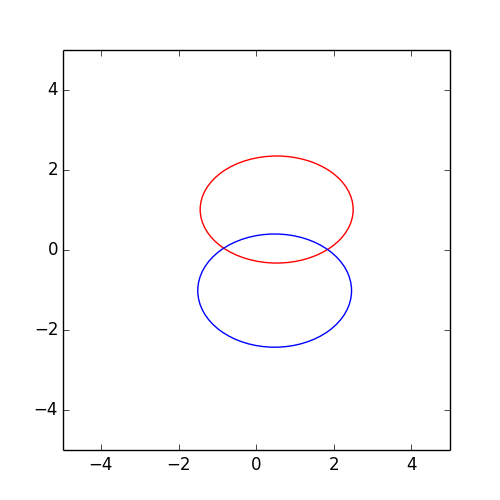
\includegraphics[width = 0.48\textwidth]{GNB_A.png}  \\
\text{ (A) Data} &  \text{ (B) } \\
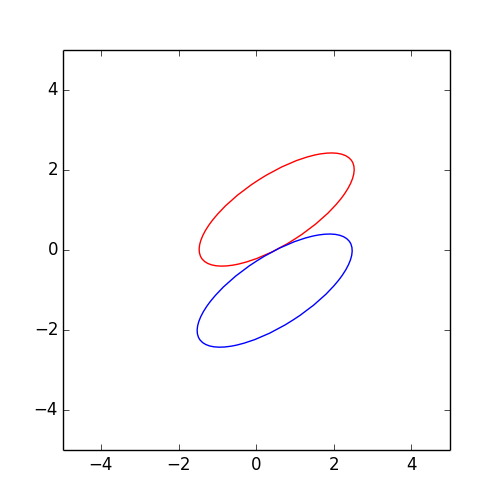
\includegraphics[width = 0.48\textwidth]{GNB_B.png} &
\includegraphics[width = 0.48\textwidth]{GNB_C.png} \\
\text{ (C)} &\text{(D)} \\
\end{tabular}
\caption{Figure of Q5 (c)}\label{fig:GNB}
\end{figure}
\maxmarks{3} \vspace{3 cm}

\clearpage

\question{6}{Text classification using Naive Bayes. (TA:- \myfirstta \& \mysecondta)}
In this assignment, you are going to program a naive Bayes classifier to classify documents from a serious European magazine ``economist'' (Class 1) and  a not-so-serious American megazine ``the onion'' (Class 0). \\
\begin{enumerate}

\item \textbf{Data description}\\
All data files are in \texttt{Onion\_vs\_Economist}.  
If you load the \texttt{handout.mat} into Octave (or Matlab) with
\texttt{load ’handout.mat’}, you will see the following matrices, 
\texttt{Xtrain,  Ytrain,  Xtest, Ytest}.
We also provided a dictionary of $V$ tokens (or words) in \texttt{dictionary.mat}, and denote the tokens in the dictionary by indices, $\{ 1,2, \cdots, V \}$.
There are $n$ training documents and $m$ testing documents. 
For each document, we counted the number of occurrence of each token, resulting in a vector $(c_1, c_2, \cdots, c_V)$. 
Each row in \texttt{Xtrain}  and \texttt{Xtest} is such a vector for one document. 
\texttt{Ytrain} and \texttt{Ytest} are $n\times 1$ and $m\times 1$ 
binary class labels.

\iffalse
\item \textbf{Model description (Binomial model)}\\
Given a document in one class with label $Y=y$, we assume a binomial distribution for each word. 
For the $i$th word in the dictionary, $W_i = 1$ denotes that the word $i$ is present in the document, where as $W_i = 0$ denotes that the word $i$ is absent.  

With a naive Bayes model, we assume that the $V$ words are independent given the class label. 
Therefore the posterior probability is 
\begin{align*}
\Pr(Y = y |W_1, \cdots, W_q) \propto \prod_{i=1}^{V} \Pr( W_i| Y = y) \Pr( Y = y)
\end{align*}
Without smoothing,
\begin{align*} 
\Pr( W_i = 1 | Y = y) = \frac{  \text{ number of documents where the $i$th word is present in Class y }} { \text{ number of documents in Class y}} 
\end{align*}
You need to use additive smoothing
http://en.wikipedia.org/wiki/Additive\_smoothing in your implementation. \\
In addition, to avoid multiplying very small probabilities and underflow, you should use a logarithmic transformation to determine the predicted class label. 

\begin{align*}
 y^* & = \arg\max_y \Pr(Y = y |W_1, \cdots, W_V)  \\
     & =  \arg\max_y  \prod_{i=1}^{V} \Pr( W_i| Y = y) \Pr( Y = y)\\
     & =  \arg\max_y  (\sum_{i=1}^{V} \log \Pr( W_i| Y = y) + \log \Pr( Y = y)))
\end{align*}
\fi

\item \textbf{Model description (multinomial model)}\\
We view a document as an ordered sequence of word events. 
Suppose we have a document with label $Y=y \in \{0,1\}$, which contains $q$ words in total, we use the event $W_i = j$ to denote the event that the $i$th word is the $j$th token in the dictionary, $j \in \{ 1,2, \cdots, V \}$. 
With a naive Bayes model, we assume that the $q$ word events are independent, and have an identical multinomial distribution with $V$ outcomes. 

\textbf{Learning the conditional probability}\\
Given one training document in Class $y$, if we do not use smoothing ( or pseudocounts ), we estimate the conditional probability for a word event $W$ in the following way,
\begin{align*}
\Pr( W = j| Y = y)  &= \frac{ \text{ number of occurrence of token $j$}}{ \text{ total number of words }} \\
&  = \frac{ \text{ number of occurrence of token $j$}}{ \text{ total number of occurrence of all $V$ tokens  }}
\end{align*}
In \texttt{Xtrain}, you are given multiple training documents in one class, you should think in a way as concatenating them all into a large document. 
You need to use additive smoothing (or pseudocount)
http://en.wikipedia.org/wiki/Additive\_smoothing in your implementation, setting $\alpha = 1$. \\

\textbf{Learning the prior}\\
Assume the prior distribution of label $Y$ is binomial, without smoothing, it is estimated as 
\[ \Pr(Y = y) = \frac{ \text{number documents in Class y}} { \text{total number of documents}}\] 


\textbf{Making prediction}\\
Now given the test document of length $q$, 
\begin{align*}
y* &= \arg\max_y \Pr(Y = y |W_1, \cdots, W_q)  = \arg\max_y \frac{ \prod_{i=1}^{q} \Pr( W_i| Y = y) \Pr( Y = y)}{ \Pr (W_1, \cdots, W_q)} \\
& = \arg\max_y (\prod_{i=1}^{q} \Pr( W_i| Y = y) \Pr( Y = y)) 
\end{align*}
However, we are only given the word counts of the document, $(c_1, c_2, \cdots, c_V)$,  and we can only compute the multinomial probability.
\begin{align}
y* &= \arg\max_y (  q! \prod_{j = 1}^{V} \frac{\Pr(W = j| Y=y)} {c_j!} \Pr( Y = y) \\ 
   & = \arg\max_y (\sum_{i=1}^{V} \log \Pr(W = j| Y=y) + \log \Pr(Y= y)) + \log (q!) - \sum_{i=1}^{V}\log(c_j!) \\ 
   & = \arg\max_y (\sum_{i=1}^{V} \log \Pr(W = j| Y=y) + \log \Pr(Y= y)) + \text{constant} \label{eq:log}
\end{align}
In your implementation, to avoid multiplying very small probabilities 
and underflow, you should use the logarithmic transformation 
as in Equation~\ref{eq:log}. 
\end{enumerate}
 
For \part{a}  submit your m-files to autolab. 
For \part{b} and \part{c}, write your solutions in your pdf. 


\part{a} Create following three octave functions and save them in three 
files, \texttt{nb\_train.m}, \texttt{nb\_test.m} and \texttt{nb\_run.m}.
\begin{verbatim}
model = nb_train(Xtrain, Y_train)
Pred_nb = nb_test(model, Xtest)
accuracy = nb_run(Xtrain, Ytrain, Xtest, Ytest)
\end{verbatim}
\texttt{model} is a structure that describe the model you learned. 
\texttt{Pred\_nb} is a $m\times 1$ binary vector, which denotes your prediction for the testing documents. 
In \texttt{nb\_run}, return the prediction accuracy  computed by \texttt{accuracy = mean(Pred\_nb==Ytest)} , and use \texttt{save('Pred\_nb.mat','Pred\_nb')} to save your prediction into a 
mat file. \\

\textbf{Note:} Your score will be determined by your classification 
accuracy on the test dataset you've been given as well as the held-out 
dataset that has not been released.

\maxmarks{15}
\part{b} For the $j$th token in the dictionary, we can compute the following log-ratio,
\[
\left |\log \frac{Pr(W = j | Y = 1) }{Pr(W = j | Y = 0)} \right|
\]
Use this log-ratio as a measure, find the top five words that are most 
discriminative of the classes, report them in your pdf. 

 
\maxmarks{5} 
\part{c}  State the Naive Bayes assumption. 
Are there any pairs of words that violate the Naive Bayes assumption? 
If so, give 1 example of such pairs and explain why they might be 
violating the Naive Bayes assumption. 
\maxmarks{5}

\dumptotal

\end{document}

